\documentclass[12pt,a4paper]{article}
\usepackage[slovene]{babel}
\usepackage[utf8]{inputenc}
\usepackage{amsmath}
\usepackage{amsthm}
\usepackage{graphicx}
\usepackage{mdframed}
\usepackage{float}

\theoremstyle{definition}
\newenvironment{zgled}{%
  \begin{mdframed}[linewidth=0.5pt, topline=true, bottomline=true, leftline=true, rightline=true, 
                  innertopmargin=\baselineskip, innerbottommargin=\baselineskip]%
  \textbf{Zgled.}%
}{%
  \end{mdframed}%
}

\begin{document}

\setlength{\parskip}{1em}
\setlength{\parindent}{0pt}

\tableofcontents

\section{Teoretični del}

\subsection{Uvod}

V javnem sektorju, za razliko od zasebnega, profitabilnost
ni tako zelo pomembna. Pogosto njeno vlogo zamenja učinkovitost. 
Učinkovitost je stopnja pri kateri je zagotavljanje storitev maksimizirana pri omejenih 
virih. Včasih je merjena tudi obratno -- kot stopnja, pri kateri je uporaba virov 
minimizirana pri pogoju zadostne zagotovitve storitev. 

Javni sektor je pogosto obravnavan kot neučinkovit zaradi odsotnosti
tekmovanja na trgu. Pričakovanja nam pravijo, da v primeru, ko obstajata
javna in zasebna storitev, bo javna manj učinkovita. To razmišljanje tudi
spodbuja gibanja v smer privatizacije javnih storitev v številnih državah.
Vendar je pomembno omeniti, da pogosto ne primerjamo primerljivih
storitev med javnim in zasebnim sektorjem. Namreč 
pogosto država zagotavlja blago in storitve ravno tam, kjer je trg odpovedal.
\cite{Lovell2002}

Vlade lahko zagotavljajo osnovne socialne storitve na področjih
zdravstva, izobraževanja in varnosti. Te storitve se financirajo
iz državenga proračuna (ki se financira iz davkov ter državenga
dolga) in ne prek zaračunavanja storitev. 

Številne študije so pokazale, da tako organizacije iz tako javnega
kot tudi zasebnega sektorja ne uporabljajo svojih omejenih virov
učinkovito. Možna posledica je, da bi prerazporeditev virov iz
zagotavljanja blaga in storitev, ki imajo razmeroma nizke
mejne družbene koristi, k tistim z razmeroma visokimi mejnimi
družbenimi koristmi, izboljšala splošno družbeno blaginjo.
Druga posledica je, da viri niso uporabljeni na najbolj 
produktiven način; to pomeni, da je mogoče proizvesti več
blaga in storitev brez dodatnih virov. \cite{Yaisawarng2002}

\subsection{Konceptno ogrodje}

Vladne agencije običajno vključujejo več enot za izvajanje 
storitev, ki zagotavljajo osnovne socialne storitve. 
Primer take delitve lahko vidimo na sliki 
\ref{fig:government_structure}.


\begin{figure}[htbp]
    \centering
    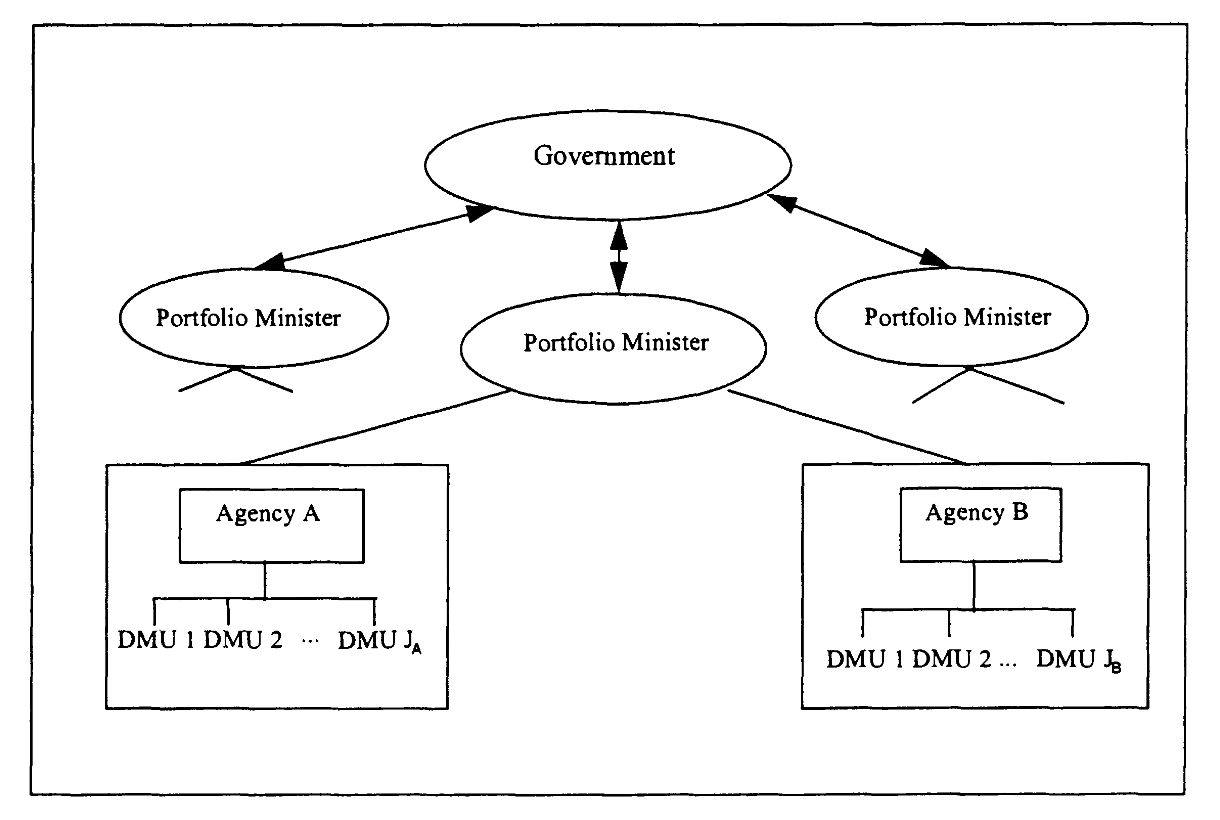
\includegraphics[width=0.7\textwidth]{government_structure.png}
    \caption{Struktura agencij v splošnem vladnem sektorju}
    \label{fig:government_structure}
    \vspace{0.2em}
    \footnotesize{Vir: \cite{Lovell2002}}
\end{figure}

Agenciji $A$ in $B$ sta odgovorni za zagotavljanje vladnih storitev, 
na primer ministrstvo za šolstvo (osnovno in srednješolsko 
izobraževanje) ter ministrstvo za delo (poklicno izobraževanje).
Agencija A vključuje $J_A$ osnovnih in srednjih šol, Agencija B 
pa $J_B$ izobraževalnih centrov. Delovanje teh agencij nadzoruje
pristojni minister. \cite{Yaisawarng2002}

\subsection{DEA analiza}

Analiza podatkovne ovojnice (\emph{angl.\ data envelopment analysis -- DEA}) je 
metoda linearnega programiranja, ki ustvari proizvodno mejo iz 
najproduktivnejših opazovanj v vzorcu. Ta meja predstavlja 
dejansko najboljšo prakso v naboru vključenih enot odločanja
(\emph{angl. decision making unit -- DMU}) in ne le teoretičnega optimuma. Ocena učinkovitosti 
vsake opazovane enote se izračuna glede na to mejo najboljše 
prakse. Ta postopek nam omogoča primerjavo uspešnosti različnih
enot, ki izvajajo podobne naloge, z najboljšimi izvajalci
v vzorcu. \cite{Yaisawarng2002}

Indeks učinkovitosti DEA je sestavljena mera uspešnosti,
ki upošteva vse vhodne in izhodne podatke v modelu ter služi
kot dopolnilno orodje k obstoječim meram produktivnosti,
kot npr.\ proizvod na delavca. Ocena učinkovitosti DEA
kaže delež trenutnih vhodov, ki
bi jih enota uporabila, če bi bila produktivno učinkovita,
ter nakazuje, ali se lahko določen vhod dodatno zmanjša brez
zmanjšanja drugih vhodov pri dani ravni izhodni vrednosti,
obenem pa zagotavlja nabor uteži, ki se uporabljajo za
oblikovanje ciljne točke za neučinkovito enoto. \cite{Yaisawarng2002}


\begin{figure}[htbp]
    \centering
    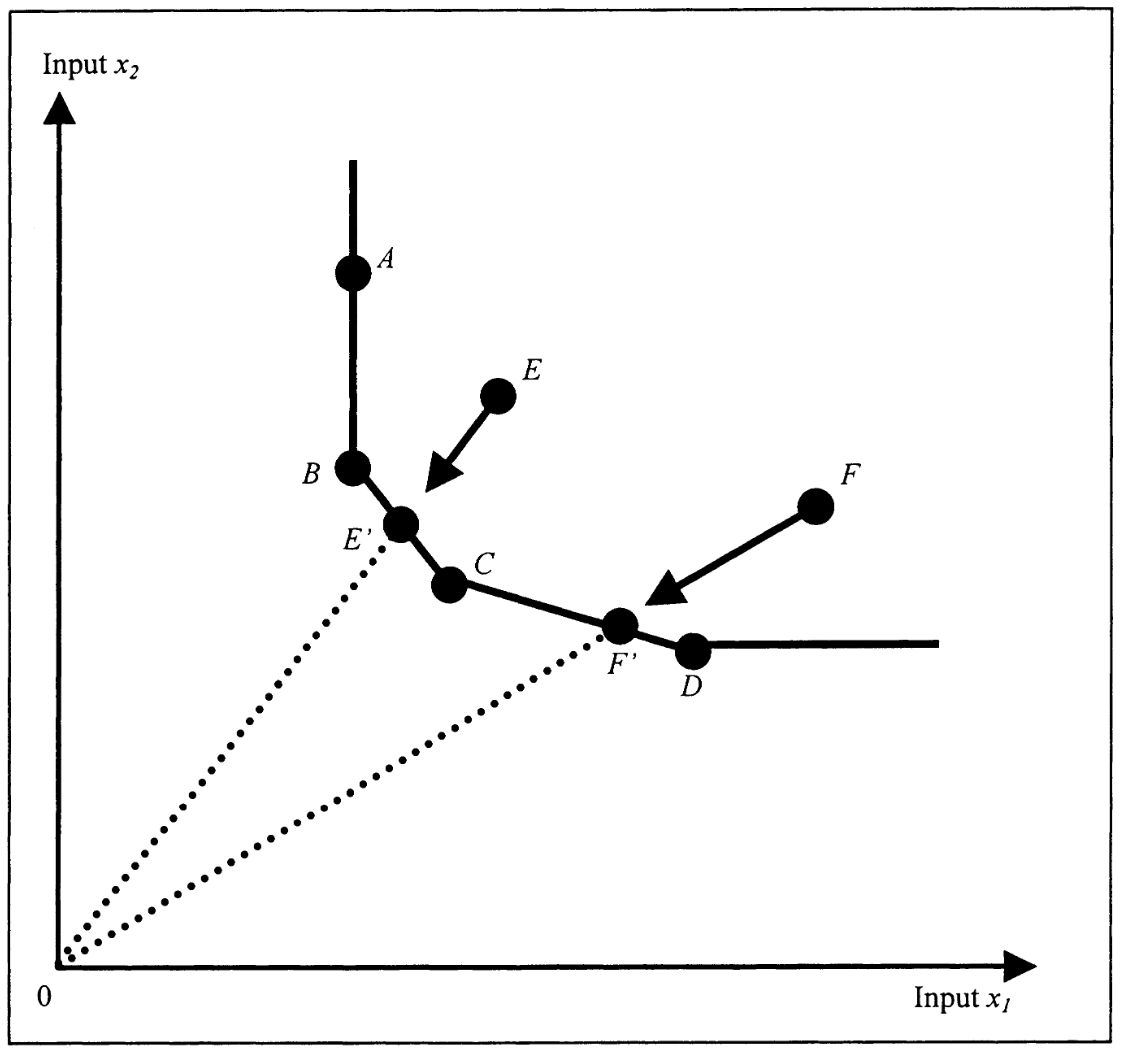
\includegraphics[width=0.7\textwidth]{dea_frontier.png}
    \caption{Proizvodna meja DEA}
    \label{fig:dea_frontier}
    \vspace{0.2em}
    \footnotesize{Vir: \cite{Lovell2002}}
\end{figure}

Slika \ref{fig:dea_frontier} predstavlja učinkovitost pri 
varčevanju z vložki za agencijo, sestavljeno iz šestih
DMU-jev, od $A$ do $F$. Vsak DMU proizvede enako količino
proizvoda $y$ pri uporabi različnih količin $x_1$ in $x_2$.
Za neučinkovit DMU $F$ velja $0F' < 0F$, oz.\ $0F'/0F < 1$,
kajti $F'$ je bližje izhodišču kot $F$. Če $F$ postane 
učinkovit, ob ohranitvi enakega razmerja vložkov, bo
na točki $F'$. Primera učinkovitih DMU-jev pa sta $C$
in $D$, ki imata višje razmerje med $y$ in $x_1$ ter
$x_2$, torej višje razmerje med vhodi in izhodi.

V tem primeru bi moral vodja neučinkovitega DMU-ja uporabiti
rezultate DEA kot vodilo pri razvoju načrta za izboljšanje
učinkovitosti. Postopek se začne z notranjo preiskavo DMU
za identifikacijo možnih razlag za prekomerno uporabo vhodnih sredstev.
Ta lahko identificira situacije, ki so specifične za ta DMU
in so zunaj nadzora vodje. V tem primeru se morajo te situacije
izvzeti iz DEA modela. Navedli bomo postopek, kako se DEA
lahko uporabi za izboljšanje učinkovitosti. \cite{Yaisawarng2002}

\begin{enumerate}
    \item Uporabimo ocene učinkovitosti DEA in tako poiščemo
    vse neučinkovite DMU-je in obseg potencialnih izboljšav. 
    Identificiramo tudi učinkovite DMU-je, primerne za 
    primerjavo in specifična področja za preiskavo.
    
    \item Izvedemo preiskavo neučinkovitega 
    DMU-ja, da lahko določimo vzroke prekomerne 
    uporabe vhodnih sredstev.
    
    \item Posvetujemo se z primerljivimi učinkovitimi DMU-ji
    o njihovih koristnih praksah.
    
    \item Analiziramo kvalitativne in kvantitativne informacije
    iz preiskave in upoštevamo uteži primerjalnih enot DEA.
    
    \item Oblikujemo strateški načrt za implementacijo v 
    neučinkovitem DMU-ju. To lahko zahteva prestrukturiranje 
    organizacije in spremembe v upravljanju. \cite{Yaisawarng2002}
\end{enumerate}

\subsection{Uporaba DEA pri alokaciji sredstev}

Ocena učinkovitosti DEA se lahko uporablja pri razvoju
omejitev financiranja za vsak DMU. V primeru, ko cene
vložkov ne odražajo celotnih ekonomskih stroškov proizvodnje
(npr.\ zaradi državnih subvencij), lahko kot kazalnik 
uspešnosti raje uporabimo tehnično učinkovitost. 
\cite{Yaisawarng2002}

\begin{zgled}
    Oglejmo si triletni model odločanja. Odločamo se o količini sredstev, ki jih bo dobil DMU $A$. Predpostavimo, da so informacije o uspešnosti za 1.\ leto na voljo v 2.\ letu, preden se odločimo za proračun za 3.\ leto.

    Najprej predpostavimo, da je pričakovana raven
    zagotavljanja storitev za 3.\ leto enaka kot v 1.\
    letu. Prav tako predpostavimo, da poznamo ocene
    učinkovitosti za vse DMU-je v 1.\ letu. Za
    zagotavljanje storitev na učinkovit način lahko vsak
    DMU zaprosi za financiranje, ki je enako stroškom tehnično
    učinkovite ali najboljše prakse kombinacije vložkov.
    Denimo, da ima DMU $A$ proračun \$300{,}000 in oceno
    tehnične učinkovitosti enako 0{,}92. To pomeni, da bo v
    3.\ letu pričakovano, da $A$ uporabi kombinacijo vložkov
    najboljše prakse in zato dobi proračun $0{,}92 \times \$300{,}000 =
    \$276{,}000$.

    Dopustimo sedaj še spremembo povpraševanja po obstoječih
    storitvah. Dodatne storitve morajo biti zagotovljene
    z uporabo vložkov najboljše prakse. Predpostavimo,
    da se je povpraševanje po storitvah DMU $A$ povečalo
    za 10 odstotkov. Tedaj mora DMU $A$ prejeti dodatna
    sredstva v višini \$27{,}600 za prilagoditev 
    pričakovani rasti povpraševanja. Denimo, da je
    ocena dodatnih stroškov zaradi povečanega
    povpraševanja \$35{,}000. V tem primeru potrebuje
    DMU $A$ skupno $\$276{,}000 + \$27{,}600 + \$35{,}000
    = \$338{,}600$.
    
    Če seštejemo prošnje za financiranje po vseh DMU-jih
    znotraj agencije $r$, dobimo najmanjšo količino sredstev,
    ki jih potrebuje. \cite{Yaisawarng2002}
\end{zgled}

Vlada razporeja razpoložljive vire vsem agencijam 
javnega sektorja glede na svoje prioritete. Če so
skupna potrebna sredstva manjša od $\$X_B$, ki je na
voljo, lahko vlada ali ministri predlagajo nove 
programe ali naložbe. Nasprotno, če potrebna sredstva
presegajo $\$X_B$, kar je bolj običajno, vlada
zahteva, da ministri znotraj DMU-jev opravijo revizijo
in tako določijo pomembnejše naloge glede na prioritete
vlade ter potrebe skupnosti. Ta proces se ponavlja,
dokler se potrebna sredstva ne zmanjšajo pod $\$X_B$.

Alternativno lahko vlada uvede splošno zmanjšanje, ali
pa zahteva od agencij, da povečajo svojo učinkovitost.
Tako nekatere agencije prejmejo manj kot potrebujejo.
V takem primeru mora agencija $r$, ki je soočena z 
zmanjšanjem svojih sredstev, uporabiti splošno
zmanjšanje za vse DMU-je znotraj te agencije. To
pomeni omejitev nekaterih storitev in preklic
izvajanja novih. \mbox{Yaisawarng} predlaga, da
prilagoditve ravni storitev znotraj DMU-jev odobri
odgovorna agencija, skupne prilagoditve za agencijo
pa odobri vlada. Predlagani proces lahko ustvari 
pritisk na DMU, da poskušajo učinkovito uporabiti 
razpoložljive vire. 
\cite{Yaisawarng2002}

Oglejmo si različne načine za določanje ciljev DMU-jev.

\begin{table}[H]
    \centering
    \caption{Možne učinkovite kombinacije vhodov}
    \label{table:dmu_primer}
    \begin{tabular}{|l|c|c|c|}
    \hline
    & $A$ & $B$ & $C$ \\
    \hline
    Izhod/Vhod 1 & 14,3 & 16,7 & 12,5 \\
    Izhod/Vhod 2 & 5,7 & 5,0 & 6,7 \\
    Vhod 1/Vhod 2 & 0,4 & 0,3 & 0,53 \\
    \hline
    \end{tabular}
    \\ \vspace{0.2em}
    \footnotesize{Vir: \cite{Yaisawarng2002}}
\end{table}
    
\begin{enumerate}
    \item[Možnost 1:] Ciljna ocena učinkovitosti za 
    DMU $A$ v 3.\ letu je najmanj 0{,}875, razmerja 
    izhod/vhod 1 in vhod 2 so najmanj 14,3 oziroma 5,7.
    
    \item[Možnost 2:] Ciljna ocena učinkovitosti za DMU
    $A$ v 3.\ letu je med 0{,}83 in 0{,}92, razmerje 
    izhod/vhod 1 je med 14,3 in 16,7, razmerje izhod/vhod 
    2 je med 5{,}7 in 6{,}7.
    
    \item[Možnost 3:] Ciljna ocena učinkovitosti za DMU
    $A$ v 3.\ letu je med 0{,}83 in 0{,}92, razmerje 
    izhod/vhod 1 je med 13{,}6 in 15, razmerje 
    izhod/vhod 2 je med 5{,}4 in 6{,}0.
\end{enumerate}

Tabela \ref{table:dmu_primer} predstavlja primer za ilustracijo
treh možnih alternativ za določanje primerjalnih
ciljev. Predpostavljamo, da DMU-ji uporabljajo dva
vhoda za proizvodnjo enega izhoda. Naj bo $A$ neučinkovit
DMU z radialno oceno učinkovitosti 0{,}875 v letu 1.
Poleg tega ima dva učinkovita vrstnika, imenovana 
$B$ in $C$. Možnost 1 določa ciljne delne mere za DMU
$A$ v 3.\ letu pri najboljši praksi kombinacije vložkov
$A$-ja glede na tehnologijo v letu 1. Te cilji 
predpostavljajo da $A$ lahko doseže stopnjo
izkoriščanja vložkov najboljše prakse pri konstantnem
razmerju tretnutnih vložkov. Ker je cilj učinkovitosti
postavljen na trenutni ravni vendar z višjim razmerjem
izhod-vhod, to pomeni, da se je proizvodna meja (Slika
\ref{fig:dea_frontier}) premaknila, kar pomeni tehnološki
napredek. \cite{Yaisawarng2002}

Možnosti 2 in 3 se od možnosti 1 razlikujeta v tem, da
določata primerjalne cilje kot interval in ne le kot točke.
Če predpostavimo, da agencija uporablja 5-odstotni pas 
dopustnih vrednosti, dobimo torej zaželeno vrednost 
učinkovitosti v letu 3 za $A$ med 0{,}83 in 0{,}92.
Možnost 2 se razlikuje še v tem, da uporablja
izhod-vhod razmerje na proizvodni meji DEA kot
spodnjo mejo ter večjega izmed razmerij učinkovitih
vrstnikov za zgornjo mejo. Možnost 3 uporabi 5-odstotni
pas okoli vrednosti na proizvodni meji DEA. 
\cite{Yaisawarng2002}

\subsection{Pomankljivosti DEA}

Seveda DEA model ne more vedno zajeti vseh pogledov
delovanje DMU-jev. Težava je lahko nedostopnost
podatkov ali pa napačna opredelitev modela.
Prav tako DEA ne dopušča šuma ali napak v podatkih.
Poleg tega se lahko zgodi, da so nekateri DMU-ji v
posameznem letu zelo učinkoviti zaradi sreče, ali pa
nasprotno, da zaradi težav zunaj njihovega nadzora
ne delujejo z največjim potencialom.

Model tudi predpostavlja, da lahko DMU-ji že skozi
proračunsko leto izboljšajo svojo učinkovitost. V
resnici potrebujejo ponavadi več obdobij za prilagoditev
in učenje. 

Preučimo lahko tudi predpostavko, da lahko z gotovostjo
napovemo rast povpraševanja na nekaterih področjih. Če
dejanska rast presega predvideno in bo DMU lahko vseeno
proizvajal na tej ravni brez dodatnih virov, ga bo
model označil za manj učinkovitega. Alternativno bi
lahko potrebovali dodatna sredstva.

Težavo lahko predstavlja tudi napredek v tehnologiji
skozi leto, ki ni bil napovedan v modelu. Kot posledico
lahko pomeni, da DMU-ji brez težav dosežejo svoje cilje,
ne da bi dejansko opravili potrebne spremembe. Zato se
mora rast tehnologije in produktivnosti predpostaviti 
in primerno spremeniti cilje.

Za konec omenimo še težavo v asimetriji informacij med
agencijami in vlado. Agencijam je namreč v interesu,
da zaprosijo za več sredstev, kolikor jih dejansko 
potrebujejo. 

\section{Praktični del}

\subsection{Povzetek}

Namen naše naloge je oceniti učinkovitost ameriškega in slovenskega
javne uprave ter ju med sabo primerjati. Ker je z DEA metodami smiselno
primerjati le DMU-je znotraj posameznih sektorjev, bomo v nalogi obravnavali le
javno zdravstvo in javno šolstvo. Za posamezen DMU bomo vzeli državo v obdobju 
treh let. Ker je vseh upravnih enot v ZDA 51 jih bomo za obravnavo izbrali le 
5 po različnosti profila: California (visok BDP in največja po prebivalstvu),
Texas (konzervativna politika, nižji javni izdatki), New York (urbana, napredno zdravstvo)
Mississipi (šibki zrdavtsveni izidi) in Utah (visoka učinkovitost). Posebej
bo obravnava tudi celotna ZDA, ki bo služila kot neke vrste "povprečje" in
posredno omogočala primerjavo z državami, ki v analizi ne bodo vključene. 

Za obdelavo vhodnih in izhodnih podatkov bomo uporabili BCC 
(Banker-Charnes-Cooper) metodo, ki se najpogosteje uporabljena za 
ocenjevanje učinkovitosti v javnih sektorjih, saj dovoljuje spremenljive 
donose, učinkovitost DMU-jev pa se ne ocenjuje le na 
absolutno produktivnost, pač pa se upošteva tudi njihova velikost.
Metoda na podlagi vhodnih in izhodnih podatkov zgradi mejo učinkovitosti (kobinacija DMU-jev,
ki so najusoešnejši), primerja vsak DMU z izračunano mejo in poda oceno od 0-1 ter 
določi vrsto obsega:

\begin{enumerate}
    \item IRS (Increasing Returns to Scale): povečanje vložkov za nek faktor vodi v povečanje
    izhoda za večji faktor,
    \item DRS (Decreasing Returns to Scale): povečanje vložkov za nek faktor vodi v povečanje
    izhoda za manjši faktor,
    \item CRS (Constant Returns to Scale): povečanje vseh vložkov za določen faktor vodi v enako povečanje izhodov.
\end{enumerate}

\nocite*{}
\bibliographystyle{apalike}
\bibliography{javni_sektor}

\end{document}
